% !TEX root = ../Ausarbeitung.tex
\section{Funktionalität von Containern}
\label{sec:Funktionalität von Container}
Container setzen direkt auf dem Kernel eines Linux-Betriebssystems auf. Um auf den Kernel durchgreifen zu können, verwenden Container standard-Linux-Techniken wie Cgroups und Namespaces oder selbst entwickelte Schnittstellen. Dadurch wird das Betriebssystem innerhalb des Containers, ohne einen Hypervisor und eine Kopie des Betriebssystems zwischen der Anwendung und der Hardware emulieren.\cite{10228802020150501} \Abbildung{linuxkernelcontainer} verdeutlicht den Kernelzugriff.
\begin{figure}[H]
	\begin{center}
		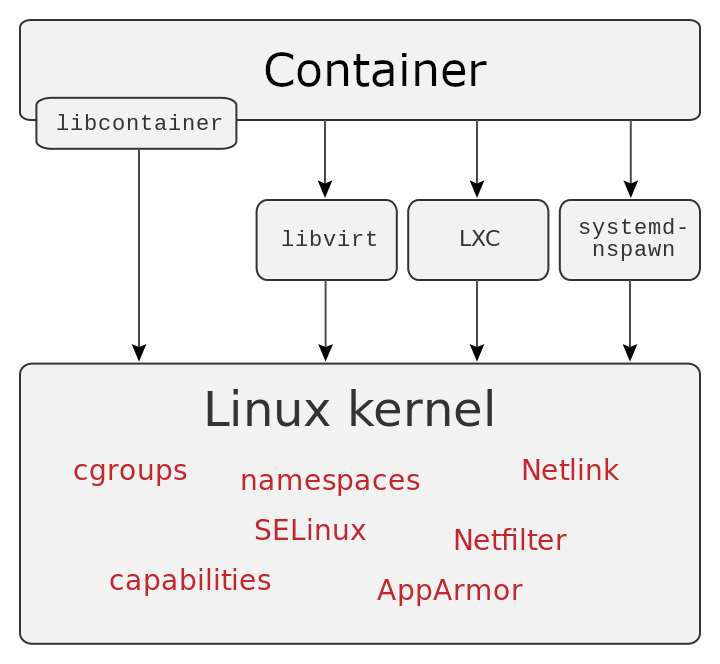
\includegraphics[width=0.7\textwidth]{LinuxKernelContainer.png}
	\end{center}
	\caption[Schnittstelle vom Container zum Kernel]{Schnittstelle vom Container zum Kernel \footnotemark}
	\label{fig:linuxkernelcontainer}
\end{figure}

\quellefoot{https://www.datacenter-insider.de/container-technik-docker-co-a-480855/index2.html}
Somit können CPU-Zyklen, Arbeitsspeicher, Blockspeicher und sonstige Schnittstellen über den Kernel angefordert und isoliert in dem jeweiligen Container zur Verfügung gestellt werden.\cite{12059254020170101}

Container sollen alles Beinhalten, was die beinhaltete Anwendung benötigt.
Die Kommunikation mit Containern funktioniert mithilfe einer virtuellen Netzwerkschnittstelle für jeden Container. Außerhalb der Container können die Ports dann gemappt werden. Natürlich kann pro Netzwerkkarte des Hosts der Port 80 nur einmal vergeben werden.\cite{10228802020150501}

Da Container nur als einzelnes Image abgelegt sind und kein Betriebssystem beinhalten, welches aktualisiert und gewartet werden müsste, beschränken sich die Installation und Deinstallation auf ein einfaches Kopieren oder Löschen des Containers. 
Aus einem Image können beliebig viele Container-Instanzen aufgerufen werden, da Schreibzugriffe nicht auf das Image zugreifen, sondern auf ein eigenes Dateisystem des Containers. Dieses Verhalten sorgt für eine sehr hohe Skalierbarkeit, da bei Bedarf einfach neue Instanzen der Anwendung gestartet werden können.\cite{12771285120180201}
Durch diese dynamische Skalierung und da die Container mit einem Bruchteil einer Sekunde im Vergleich zu VM´s oder dedizierten Servern sehr schnell gestartet und beendet werden können, haben sie eine deutlich kürzere durchschnittliche Lebensdauer. Die genaue prozentuale Verteilung der statistischen Ausführungszeiten von Containern (Dauer zwischen Containerstart und Containerende) kann der \Abbildung{Lebensdauer} entnommen werden:
\begin{figure}[H]
	\begin{center}
		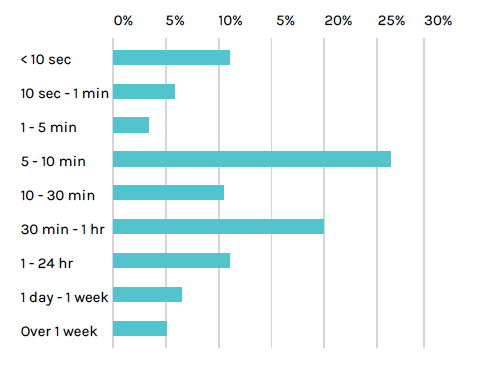
\includegraphics[width=0.7\textwidth]{Lebensdauer.png}
	\end{center}
	\caption[Lebensdauer eines Containers]{Lebensdauer eines Containers \footnotemark}
	\label{fig:Lebensdauer}
\end{figure}
\quellefoot{https://www.dailyhostnews.com/wp-content/uploads/2018/05/d3.png}
In den letzten 10 Jahren haben Container einen großen Wandel durchlebt, welcher in \Abschnitt{Containertechnologien} näher erläutert wird.
\newpage